% 图 7.4 外场 2μ_B B 下 g(E) 自旋子带劈裂示意（夸大）
\documentclass[tikz,border=5pt]{standalone}
\usetikzlibrary{arrows.meta}
\usepackage{amsmath}
\usepackage{bm}
\usepackage{fontspec}
\setmainfont{Times New Roman}
\begin{document}
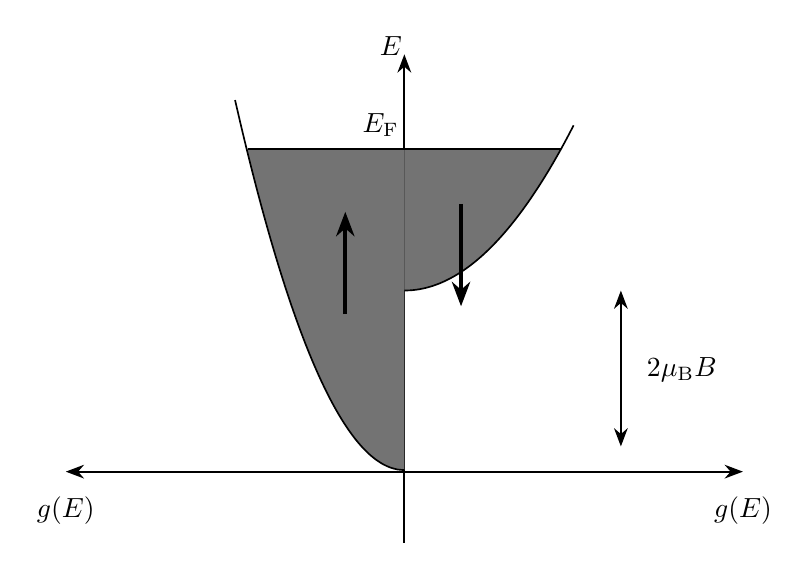
\begin{tikzpicture}[line width=0.8pt,>=Stealth]
% 底线（两端向外箭头）
\draw[Stealth-Stealth] (-4.3,0) -- (4.3,0);
\node at (-4.3,-0.5) {$g(E)$};
\node at (4.3,-0.5) {$g(E)$};
% 中央 E 轴
\draw[->] (0,-0.9) -- (0,5.3);
\node[above left] at (0.1,5.15) {$E$};
% 左带（自旋↑）：顶点在底线上，填充至 E_F=4.1
\fill[black!55] plot[domain=-2.0034:0] (\x,{0.02+1.0165*\x*\x}) -- (0,4.1) -- cycle;
\draw[line width=0.6pt] plot[domain=-2.15:0,smooth]
  (\x,{0.02+1.0165*\x*\x});
% 右带（自旋↓）：整体上移，顶点 2.3
\fill[black!55] plot[domain=0:1.989] (\x,{2.3+0.454*\x*\x}) -- (0,4.1) -- cycle;
\draw[line width=0.6pt] plot[domain=0:2.15,smooth]
  (\x,{2.3+0.454*\x*\x});
% 填充顶线（E_F）
\draw[line width=0.9pt] (-1.99,4.1) -- (1.99,4.1);
\node[above] at (-0.3,4.12) {$E_{\mathrm{F}}$};
% 自旋箭头
\draw[line width=1.3pt,->] (-0.75,2.0) -- (-0.75,3.3);
\draw[line width=1.3pt,->] (0.72,3.4) -- (0.72,2.1);
% 2μ_BB 双箭头（底线与右带顶点之间）
\draw[Stealth-Stealth] (2.75,0.32) -- (2.75,2.3);
\node[right] at (2.95,1.3) {$2\mu_{\mathrm{B}}B$};
\end{tikzpicture}
\end{document}
